\PassOptionsToPackage{unicode=true}{hyperref} % options for packages loaded elsewhere
\PassOptionsToPackage{hyphens}{url}
%
\documentclass[
]{article}
\usepackage{lmodern}
\usepackage{amssymb,amsmath}
\usepackage{ifxetex,ifluatex}
\ifnum 0\ifxetex 1\fi\ifluatex 1\fi=0 % if pdftex
  \usepackage[T1]{fontenc}
  \usepackage[utf8]{inputenc}
  \usepackage{textcomp} % provides euro and other symbols
\else % if luatex or xelatex
  \usepackage{unicode-math}
  \defaultfontfeatures{Scale=MatchLowercase}
  \defaultfontfeatures[\rmfamily]{Ligatures=TeX,Scale=1}
\fi
% use upquote if available, for straight quotes in verbatim environments
\IfFileExists{upquote.sty}{\usepackage{upquote}}{}
\IfFileExists{microtype.sty}{% use microtype if available
  \usepackage[]{microtype}
  \UseMicrotypeSet[protrusion]{basicmath} % disable protrusion for tt fonts
}{}
\makeatletter
\@ifundefined{KOMAClassName}{% if non-KOMA class
  \IfFileExists{parskip.sty}{%
    \usepackage{parskip}
  }{% else
    \setlength{\parindent}{0pt}
    \setlength{\parskip}{6pt plus 2pt minus 1pt}}
}{% if KOMA class
  \KOMAoptions{parskip=half}}
\makeatother
\usepackage{xcolor}
\IfFileExists{xurl.sty}{\usepackage{xurl}}{} % add URL line breaks if available
\IfFileExists{bookmark.sty}{\usepackage{bookmark}}{\usepackage{hyperref}}
\hypersetup{
  pdftitle={JC24533 postdoc position},
  pdfborder={0 0 0},
  breaklinks=true}
\urlstyle{same}  % don't use monospace font for urls
\usepackage[margin=1in]{geometry}
\usepackage{color}
\usepackage{fancyvrb}
\newcommand{\VerbBar}{|}
\newcommand{\VERB}{\Verb[commandchars=\\\{\}]}
\DefineVerbatimEnvironment{Highlighting}{Verbatim}{commandchars=\\\{\}}
% Add ',fontsize=\small' for more characters per line
\usepackage{framed}
\definecolor{shadecolor}{RGB}{248,248,248}
\newenvironment{Shaded}{\begin{snugshade}}{\end{snugshade}}
\newcommand{\AlertTok}[1]{\textcolor[rgb]{0.94,0.16,0.16}{#1}}
\newcommand{\AnnotationTok}[1]{\textcolor[rgb]{0.56,0.35,0.01}{\textbf{\textit{#1}}}}
\newcommand{\AttributeTok}[1]{\textcolor[rgb]{0.77,0.63,0.00}{#1}}
\newcommand{\BaseNTok}[1]{\textcolor[rgb]{0.00,0.00,0.81}{#1}}
\newcommand{\BuiltInTok}[1]{#1}
\newcommand{\CharTok}[1]{\textcolor[rgb]{0.31,0.60,0.02}{#1}}
\newcommand{\CommentTok}[1]{\textcolor[rgb]{0.56,0.35,0.01}{\textit{#1}}}
\newcommand{\CommentVarTok}[1]{\textcolor[rgb]{0.56,0.35,0.01}{\textbf{\textit{#1}}}}
\newcommand{\ConstantTok}[1]{\textcolor[rgb]{0.00,0.00,0.00}{#1}}
\newcommand{\ControlFlowTok}[1]{\textcolor[rgb]{0.13,0.29,0.53}{\textbf{#1}}}
\newcommand{\DataTypeTok}[1]{\textcolor[rgb]{0.13,0.29,0.53}{#1}}
\newcommand{\DecValTok}[1]{\textcolor[rgb]{0.00,0.00,0.81}{#1}}
\newcommand{\DocumentationTok}[1]{\textcolor[rgb]{0.56,0.35,0.01}{\textbf{\textit{#1}}}}
\newcommand{\ErrorTok}[1]{\textcolor[rgb]{0.64,0.00,0.00}{\textbf{#1}}}
\newcommand{\ExtensionTok}[1]{#1}
\newcommand{\FloatTok}[1]{\textcolor[rgb]{0.00,0.00,0.81}{#1}}
\newcommand{\FunctionTok}[1]{\textcolor[rgb]{0.00,0.00,0.00}{#1}}
\newcommand{\ImportTok}[1]{#1}
\newcommand{\InformationTok}[1]{\textcolor[rgb]{0.56,0.35,0.01}{\textbf{\textit{#1}}}}
\newcommand{\KeywordTok}[1]{\textcolor[rgb]{0.13,0.29,0.53}{\textbf{#1}}}
\newcommand{\NormalTok}[1]{#1}
\newcommand{\OperatorTok}[1]{\textcolor[rgb]{0.81,0.36,0.00}{\textbf{#1}}}
\newcommand{\OtherTok}[1]{\textcolor[rgb]{0.56,0.35,0.01}{#1}}
\newcommand{\PreprocessorTok}[1]{\textcolor[rgb]{0.56,0.35,0.01}{\textit{#1}}}
\newcommand{\RegionMarkerTok}[1]{#1}
\newcommand{\SpecialCharTok}[1]{\textcolor[rgb]{0.00,0.00,0.00}{#1}}
\newcommand{\SpecialStringTok}[1]{\textcolor[rgb]{0.31,0.60,0.02}{#1}}
\newcommand{\StringTok}[1]{\textcolor[rgb]{0.31,0.60,0.02}{#1}}
\newcommand{\VariableTok}[1]{\textcolor[rgb]{0.00,0.00,0.00}{#1}}
\newcommand{\VerbatimStringTok}[1]{\textcolor[rgb]{0.31,0.60,0.02}{#1}}
\newcommand{\WarningTok}[1]{\textcolor[rgb]{0.56,0.35,0.01}{\textbf{\textit{#1}}}}
\usepackage{graphicx,grffile}
\makeatletter
\def\maxwidth{\ifdim\Gin@nat@width>\linewidth\linewidth\else\Gin@nat@width\fi}
\def\maxheight{\ifdim\Gin@nat@height>\textheight\textheight\else\Gin@nat@height\fi}
\makeatother
% Scale images if necessary, so that they will not overflow the page
% margins by default, and it is still possible to overwrite the defaults
% using explicit options in \includegraphics[width, height, ...]{}
\setkeys{Gin}{width=\maxwidth,height=\maxheight,keepaspectratio}
\setlength{\emergencystretch}{3em}  % prevent overfull lines
\providecommand{\tightlist}{%
  \setlength{\itemsep}{0pt}\setlength{\parskip}{0pt}}
\setcounter{secnumdepth}{-2}
% Redefines (sub)paragraphs to behave more like sections
\ifx\paragraph\undefined\else
  \let\oldparagraph\paragraph
  \renewcommand{\paragraph}[1]{\oldparagraph{#1}\mbox{}}
\fi
\ifx\subparagraph\undefined\else
  \let\oldsubparagraph\subparagraph
  \renewcommand{\subparagraph}[1]{\oldsubparagraph{#1}\mbox{}}
\fi

% set default figure placement to htbp
\makeatletter
\def\fps@figure{htbp}
\makeatother

\hypersetup{colorlinks = false, pdfborder={1 1 1}}
\newcommand{\pkg}[1]{{\fontseries{m}\fontseries{b}\selectfont #1}}
\usepackage{booktabs}
\usepackage{longtable}
\usepackage{array}
\usepackage{multirow}
\usepackage{wrapfig}
\usepackage{float}
\usepackage{colortbl}
\usepackage{pdflscape}
\usepackage{tabu}
\usepackage{threeparttable}
\usepackage{threeparttablex}
\usepackage[normalem]{ulem}
\usepackage{makecell}
\usepackage{xcolor}

\title{JC24533 postdoc position}
\usepackage{etoolbox}
\makeatletter
\providecommand{\subtitle}[1]{% add subtitle to \maketitle
  \apptocmd{\@title}{\par {\large #1 \par}}{}{}
}
\makeatother
\subtitle{cover letter}
\author{Thomas Huet\\
mail:
\href{mailto:thomashuet7@gmail.com}{\nolinkurl{thomashuet7@gmail.com}}\\
website: \url{https://github.com/zoometh/}}
\date{12/8/2020}

\begin{document}
\maketitle

The University of Cambridge opens a fixed-term postdoctoral position, in
the framework of the
\href{https://www.encounterproject.info/}{ERC-funded research project
ENCOUNTER} (PI: Enrico Crema), to assess \textbf{cultural boundaries},
\textbf{cultural connectivity} and \textbf{cultural changes} during the
Jōmon-Yayoi transition period.

During more than 10,000 years, Jōmon (16,000--2,800 cal BP) maintain a
hunter-gather economy, while the surroundings of the island adopted
progressively farming economy (Habu and Junko 2004). During the Late
Jōmon and Final Jōmon phases (4,420-2,800 cal BP), Southern Yayoi
farmers introduced rice and millet to the Japan archipel. The ENCOUNTER
project plan to respond to this main question: triggered by the Yayoi
demic and cultural-trait diffusion, how the Jōmon culture changes ? To
adress this question, multiple lines of evidence coming from Japanese
excavation reports (radiocarbon dates, subsistence systems, residiential
models, mortuary/ceremonial practices, crafts/trade networks, etc.) and
new studies conducted by the project members and key collaborators
(organic residues analyses, climatic and landcover restitution, etc.)
will be analysed over the \textbf{long-term} and at a \textbf{large
geographical scale} with computational methods.

I am familiar with computational archaeology and computer-based analysis
to study archaeological traits over the \textbf{long-term} and at a
\textbf{large geographical scale}. I am used to conduct archaeological
researches with formal methods. For example, \textbf{cultural
boundaries} can be defined as the spatial extent where cultural traits
share more between them (intra-variability) than with cultural traits
outside this extent (inter-variability). These cultural traits come from
different social subsystems (subsistence, technological, demographic,
ecological, symbolic) that should be assessed with
polythetic/multifactorial analysis and computational methods with
descriptive statistics, data mining and statistical test at the temporal
and spatial scales. I assume that \textbf{cultural connectivity} and
\textbf{cultural change} should be model with the same statistical
means.

Regarding the \textbf{spatial dimension}, data coming from organic
residue analysis (WP2), land cover restitution (WP4) and
archaeobotanical (WP5) will be processed with map algebra to contrast
Jōmo regional responses to the Yayoi economic spreading. I am used to
manage spatial analysis such as: sitology, site catchment analysis,
shorter paths, inter-visibilities, etc., and to deal with spatial
auto-correlation, point pattern analysis, etc. Regarding the
\textbf{temporal dimension}, it is hard to consider the whole Jōmon
period as a unitary culture since, at least, three cycles of population
have been percieved (Kobayashi 2008). A great insight will be to
parallelized radiocarbon dates summed probability distribution (SPD)
with the Jomon well-documented pottery typo-chronology and other
cultural-traits (Habu 2008; Crema and Kobayashi 2020). I am familiar
with SPDs (see for example the RShiny
\href{https://neolithic.shinyapps.io/Euroevol_R/}{EUROEVOL\_R app}) and
cultural-traits seriations (ie typo-chronology). I am also used to
manage interval temporal logic, like Allen's formalism, with
computer-based methods. In such a modeling, \emph{events} are considered
as \texttt{POINTS} when \emph{duration} as considered as \texttt{LINES}
with a starting \emph{event} (x\textsuperscript{-}) and an ending
\emph{event} (x\textsuperscript{+}). Durations and events can be manage
with binary topological relationships (\emph{birel}) and operators like
touches/meets, overlaps/intersects, etc.

I mostly use methods like database/GIS and programmed routines of
spatial and non-spatial statistical analysis with \textsf{R}. I also
manage networks analysis either for spatial and non-spatial data. In a
context of Open Science, open data, and Digital Humanities, I also
manage content management system (CMS), GeoCMS, data sharing, data
vizualisation with enriched charts and web interactive forms (see the
\href{https://zoometh.github.io/golasecca/}{Golasecca-net webpage} for
spatial and non-spatial networks, and JSON\_LD serialization).

I am also able to find, access, interoperate and reuse (FAIR) data, like
those published as supplementary material and hosted on the GitHub
\href{https://github.com/ercrema/jomonPhasesAndPopulation}{\textbf{\emph{Jomon\_SPD\_Comparison}}
repository}, with near 2,000 radiocarbon dates (Crema and Kobayashi
2020) can be connected, read, calibrated and plotted with \textsf{R} and
the packages \pkg{curl} and \pkg{rcarbon} (Ooms 2019; Bevan and Crema
2020)\\
\hspace*{0.333em}

\begin{Shaded}
\begin{Highlighting}[]
\KeywordTok{library}\NormalTok{(curl) }\CommentTok{# to connect url}
\KeywordTok{library}\NormalTok{(rcarbon) }\CommentTok{# for C14 calibrations}
\NormalTok{gh.repo <-}\StringTok{ "https://raw.github.com/ercrema/Jomon_SPD_Comparison/"}
\NormalTok{gh.c14 <-}\StringTok{ "master/data/c14dates.csv"}
\NormalTok{gh.data.c14 <-}\StringTok{ }\KeywordTok{read.csv}\NormalTok{(}\KeywordTok{curl}\NormalTok{(}\KeywordTok{paste0}\NormalTok{(gh.repo, gh.c14)))}
\NormalTok{gh.data.c14.sample <-}\StringTok{ }\KeywordTok{head}\NormalTok{(gh.data.c14) }\CommentTok{# first dates}
\NormalTok{gh.data.c14.sample}\OperatorTok{$}\NormalTok{ids <-}\StringTok{ }\DecValTok{1}\OperatorTok{:}\KeywordTok{nrow}\NormalTok{(gh.data.c14.sample)}
\NormalTok{ages <-}\StringTok{ }\KeywordTok{calibrate}\NormalTok{(}\DataTypeTok{x =}\NormalTok{ gh.data.c14.sample}\OperatorTok{$}\NormalTok{C14Age,}
                  \DataTypeTok{errors =}\NormalTok{ gh.data.c14.sample}\OperatorTok{$}\NormalTok{C14Error,}
                  \DataTypeTok{calCurves =} \StringTok{'intcal13'}\NormalTok{,}
                  \DataTypeTok{ids =}\NormalTok{ gh.data.c14.sample}\OperatorTok{$}\NormalTok{LabCode,}
                  \DataTypeTok{verbose =}\NormalTok{ F)}
\KeywordTok{multiplot}\NormalTok{(ages, }\DataTypeTok{decreasing=}\OtherTok{TRUE}\NormalTok{, }\DataTypeTok{HPD=}\OtherTok{TRUE}\NormalTok{)}
\end{Highlighting}
\end{Shaded}

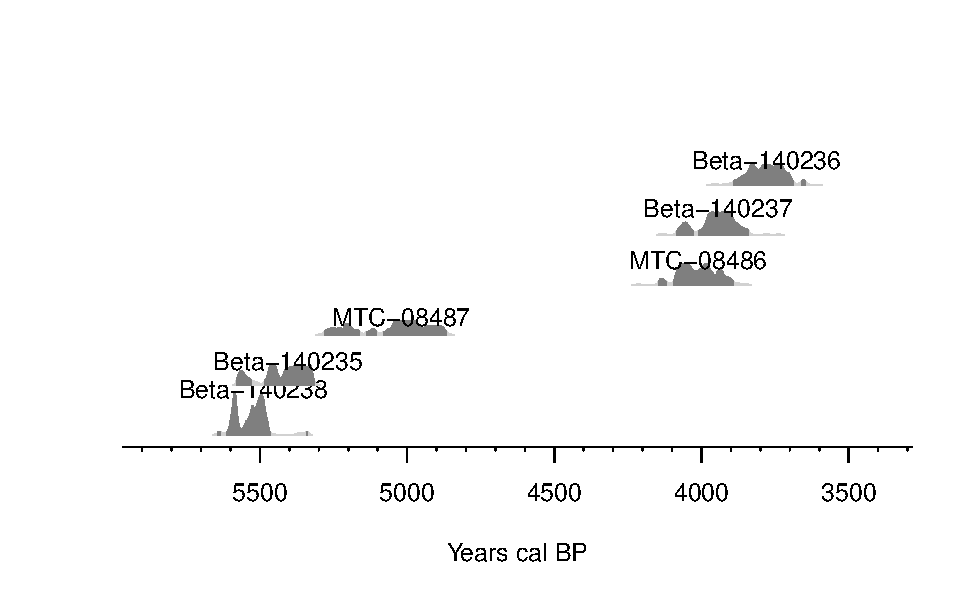
\includegraphics{index_files/figure-latex/dat-1.pdf}

The geographical counterpart of this radiocarbon dates plot -- with the
whole dataset --, made with \textsf{R} and the pakages \pkg{leaflet},
\pkg{htmltools}, \pkg{dplyr} and \pkg{curl}, can be seen on a
\href{https://zoometh.github.io/encounter_postdoc/docs/lf_jomon_sites.html}{GitHub
webpage}.

\hypertarget{last-words}{%
\subsection{Last Words}\label{last-words}}

Archaeological researches over the long-term and at a large scale, like
the ENCOUNTER project, integrate large amount of heteroclit data into
computational routines. I am used to manage and analyse data with
\textsf{R}, GIS and databases, to develop authoring frameworks for data
science like RShiny or Rmarkdown documents, Mardown and \LaTeX syntaxes.
In a context of Open Science, I also know how to manage open data
referencing and online sourcing/publishing. Regarding the archaeological
context -- even I am not familiar with the Japanese prehistory -- I have
already an experience on studying acculturation processes like for the
Mesolithic-Neolithic transition or the end of the Protohistory in
Western Europe. Working on the Jōmon-Yayoi transition will allow me to
\emph{de-focuse} my current perception of farming/innovation adoption.
It would be a great experience for me to developp IT and scientific
solutions within the frame of the ENCOUNTER research project and join a
team open to innovative methods.

\hypertarget{reference}{%
\section*{Reference}\label{reference}}
\addcontentsline{toc}{section}{Reference}

\hypertarget{refs}{}
\leavevmode\hypertarget{ref-Bevan20}{}%
Bevan, Andrew, and Enrico R. Crema. 2020. \emph{Rcarbon: Methods for
Calibrating and Analysing Radiocarbon Dates}.
\url{https://github.com/ahb108/rcarbon}.

\leavevmode\hypertarget{ref-crema2020multi}{}%
Crema, Enrico R, and Ken'ichi Kobayashi. 2020. ``A Multi-Proxy Inference
of Jōmon Population Dynamics Using Bayesian Phase Models, Residential
Data, and Summed Probability Distribution of 14C Dates.'' \emph{Journal
of Archaeological Science} 117: 105136.

\leavevmode\hypertarget{ref-Habu08}{}%
Habu, Junko. 2008. ``Growth and Decline in Complex Hunter-Gatherer
Societies: A Case Study from the Jomon Period Sannai Maruyama Site,
Japan.'' \emph{Antiquity} 82 (317): 571--84.

\leavevmode\hypertarget{ref-habu2004ancient}{}%
Habu, Junko, and Habu Junko. 2004. \emph{Ancient Jomon of Japan}. Vol.
4. Cambridge University Press.

\leavevmode\hypertarget{ref-kobayashi2008jomon}{}%
Kobayashi, K. 2008. ``Jomon-Jidai No Rekinendai.'' \emph{Rekishino
Monosashi}, 257--69.

\leavevmode\hypertarget{ref-Ooms19}{}%
Ooms, Jeroen. 2019. \emph{Curl: A Modern and Flexible Web Client for R}.
\url{https://CRAN.R-project.org/package=curl}.

\end{document}
